In our experiment, tree-aggregation algorithms are examined in multi-threading. This experiment is to evaluate the impact of having Arc (Atomic Reference Counting) as elements of vectors. 
In Big Data mining tools, such as Spark, it generates intermediate objects from the original source vector. In tree-aggregation, aggregated HashMap like data structures is created in each step or node. 
Acquisition of elements in the source vector is required to perform this aggregation. There are several ways.

One way is to deep-copy elements of the vector. This solution allocates newly created objects by deep-copy. 
Aggregation is performed on copied objects, they are stored in the data structure and sent to next node. 
Deep-copying generates duplicates of objects in vectors and aggregated data structure. 
This can lead to memory intensive moments when we need memory space for the additional duplicated objects.

The other way is to get reference to the elements. Since an original source vector is deallocated after a local aggregation,
simple references to elements do not live long enough and allow the aggregation result to be sent to next node. 
Instead of simple borrowing, we need owners in the aggregation result. Reference Counting (Rc) in Rust is a way to have multiple owners to a value. 
Since our experiment is implemented in multithreading, Arc (Arc) is used instead of Rc. With Arc, multiple ownership pointers can be 
possessed by different variables across multiple threads. Therefore, a value is not deallocated until all owners to it are dropped. 
This does not require extra memory allocation, because only acquisition of new ownership to the value is needed. 
However, as explained in the last section deletion of Arc type checks whether the value is still owned by other variables. 
This checking may be an overhead in algorithms that generate a lot of intermediate data structures, because deletion of the data structures occurs frequently.

Two algorithms are implemented using the above two methods and their runtime performance is evaluated . 
We perform aggregation to CustomerOwned based on last\_name field. 
Before tree-aggregation algorithms are run, partitions of Vec$<$CustomerOwned$>$ or of Vec$<$Arc$<$CustomerOwned$>>$ are created, serialized, and stored in disk.
A tree-aggregate algorithm has main three phases: loading, aggregating, and combining phase. 
At loading phase the algorithm generates threads. In each node, it loads serialized CustomerOwned partition from disk and deserialize them.
At aggregating phase, aggregation is performed on each partition by last\_name field. Once a node finishes aggregation, it sends result to parent node. 
After parent nodes receive aggregation results from all of its children nodes, it joins all aggregation results including its and sends to the next parent. 
This joining aggregation results is considered as combining phase. 

Two kinds of algorithms are implemented. One algorithm performs aggregation by deep-copying elements from a source vector loaded from a disk. 
In the other algorithm, each element of the source vector is wrapped in Arc, and its reference is acquired while aggregation. 
The difference between the both algorithm codes are represented in Figure~\ref{fig:arc_tree} and in Figure~\ref{fig:deep_tree}.
If we glance at the codes, the notable difference is only when we acquire an element from CustomerOwned Vec to construct an aggregated data structure.
Therefore, there are few difference between the two kinds of tree-aggregate algorithm in terms of code appearance.

Numbers of CustomerOwned objects aggregated in our experiment are 2, 4, 6, 8 million. 

\begin{figure}[htb]
    \begin{lstlisting}
        fn aggregate_local(arr :&[Arc<CustomerOwned>]) 
        {   
            let mut agg = HashMap::new();
            let n = arr.len();
            for i in 0..n {
                let customer = Arc::clone(&arr[i]);
                let last_name = customer.last_name.clone();
                let vector = agg.entry(last_name).or_insert_with(Vec::new);
                vector.push(customer);
            }
            return agg;
        }
    \end{lstlisting}
    \caption{Aggregation function with Arc}
    \label{fig:arc_tree}
\end{figure}


\begin{figure}[htb]
    \begin{lstlisting}
        fn aggregate_local_copy(arr :&[CustomerOwned]) 
        {   
            let mut agg = HashMap::new();
            let n = arr.len();
            for i in 0..n {
                let customer = arr[i].clone();
                let last_name = customer.last_name.clone();
                let vector = agg.entry(last_name).or_insert_with(Vec::new);
                vector.push(customer);
            }
            return agg;
        }
    \end{lstlisting}
    \caption{Aggregation function with deep-copy}
    \label{fig:deep_tree}
\end{figure}


\subsection{Result}
Figure~\ref{fig:ex_tree_agg} shows runtime performance of two tree-aggregate algorithms. 
The runtime of algorithm with deep-copy is about 40 to 50\% slower than algorithm with Arc for every vector size. 
The memory usage of algorithm with Arc and size of 8 million is about 15G bytes. On the other hand, 
the memory usage of algorithm with deep-copy and size of 8 million is about 26G bytes.

\begin{figure}[htb]
    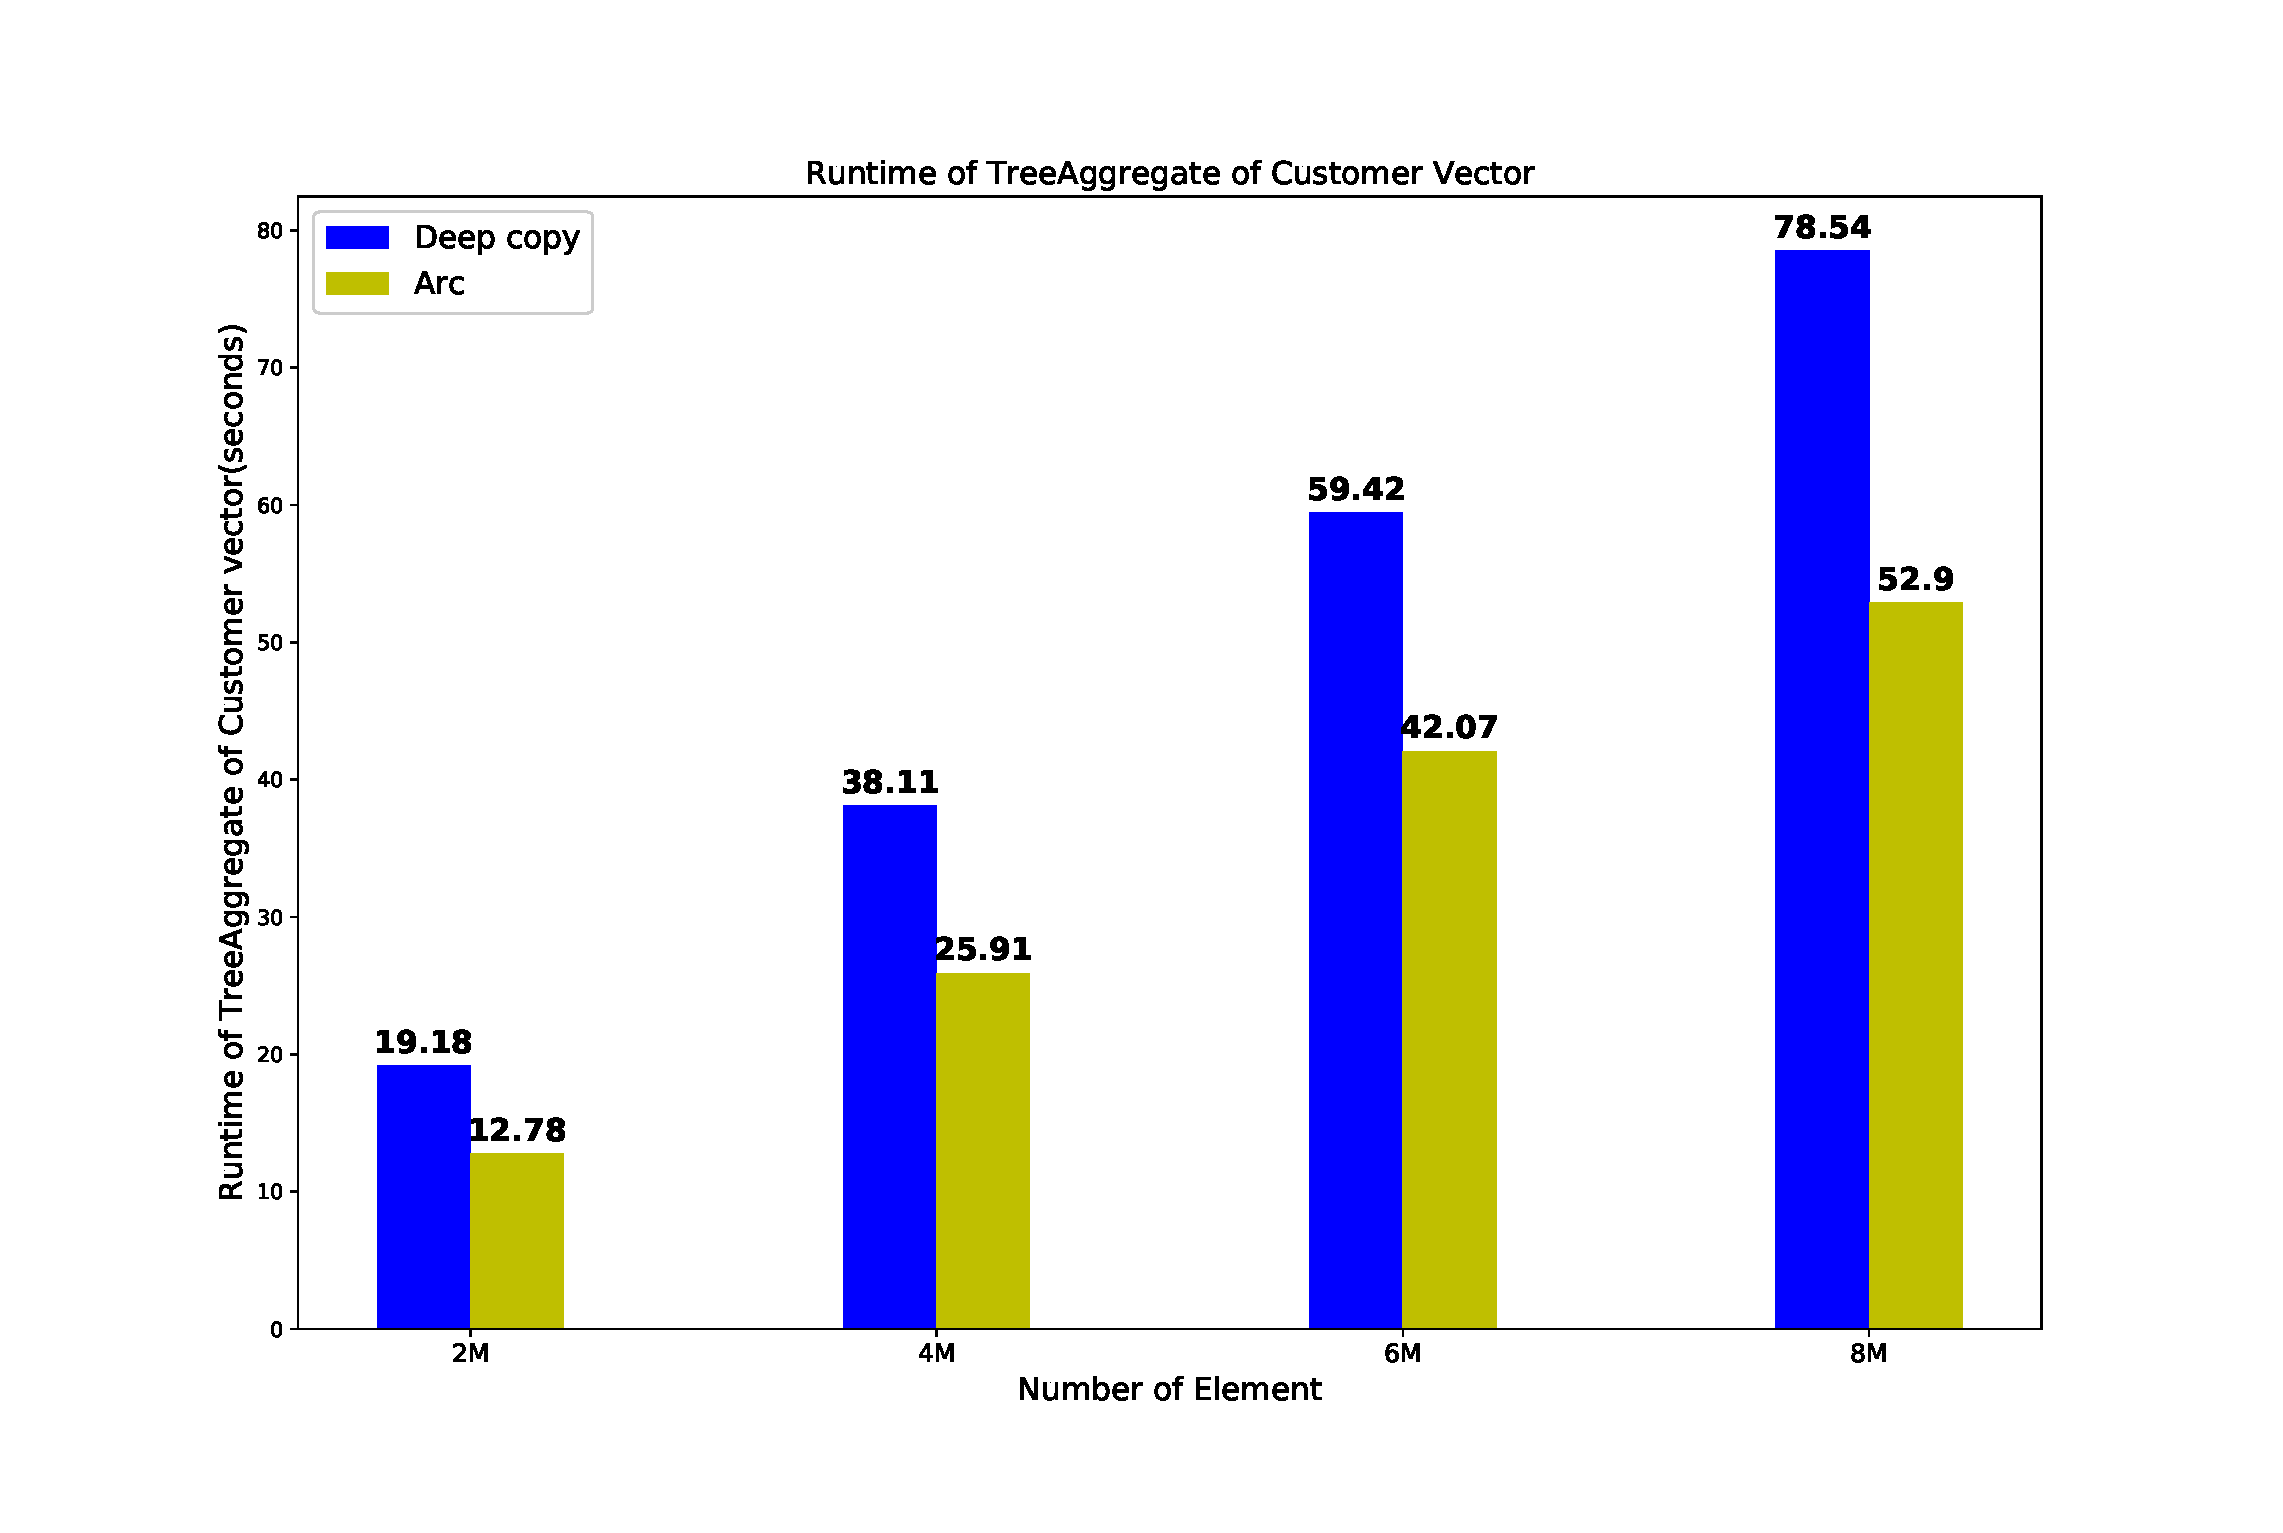
\includegraphics[width=15cm]{rust_tree_aggregate.eps}
    \caption{Runtime of Tree-aggregate algorithm}
    \label{fig:ex_tree_agg}
\end{figure}

\subsection{Discussion}
As we explained, Arc has overhead to be deleted because it has to check if the value is still referred. The atomic operations are more expensive than ordinal memory access.
Even though the use of Arc slows down runtime performance, deep copy of complex objects has more impact in deterioration of runtime performance. 

At the aggregating phase, each object is deep-copied or acquired with Arc once during the runtime in order to construct aggregated data structures.
If total number of objects is 1 million, the all of 1 million objects are deep-copied or cloned with Arc once during execution. 
Deep-copy allocates new memory for copied object. On the other hand, clone with Arc is merely acquisition of additional owner. 
Therefore, deep-copy is more expensive in terms of runtime and also use of memory than clone with Arc. 
Deep-copy processes all the original objects to generate newly deep-copied objects. 
This process has overhead and the existence of both original and copied objects doubles its memory usage.

After construction of aggregated data structure, the dropping variables of original objects occurs at the end of the aggregating phase.
In the algorithm with deep-copy, these variables are owners so that drop of variables triggers deallocation of actual values.
In the algorithm with Arc, the variables are Arc. The aggregated data structure contains Arc pointing to the same values pointed by original Arc.
Since the aggregated data structures continue to live after aggregating phase, drop of original Arcs does not triggers deallocation of values. 
Therefore, drop of original variables can shows overhead of memory deallocation in algorithm with deep-copy, 
and overhead of checking reference count of Arc in algorithm with Arc.

In addition, memory access from Arc is slower than ordinal variables due to the atomic operations. This may be potential overhead of the algorithm with Arc.

Considered these theoretical analysis and result of our experiment, using Arc improves runtime performance and memory usage compared to algorithms using deep-copy in tree-aggregate algorithms.